%\documentclass[english]{beamer}
\documentclass[english,hangout]{beamer}
%\documentclass[aspectratio=169]{beamer}
%\usepackage{amsmath}
%\usepackage{amssymb}
\usepackage{rotating}
\usepackage{verbatim}
\usepackage{latexsym}
\usepackage{graphicx}
\usepackage{tabularx}
\usepackage{ragged2e}
\usepackage{eurosym}   % Euro symbol: \euro
\usepackage{listings}
\usepackage{multirow}
\usepackage{colortbl}
\usepackage{textcomp}  % many special symbols
\usepackage{lmodern}
\usepackage{times}
\usepackage[T1]{fontenc}
\usepackage[utf8]{inputenc}
\usepackage[english]{babel}
\usepackage{booktabs}
\usepackage{setspace}


\usetheme[fb2]{FrankfurtUniversity}
%\usetheme[fb2,noslogan]{FrankfurtUniversity}
%\slogan{\large\color{red}UNAUTHORIZED}


\title{Dynamic Exercise Generation}
\subtitle{}
\author{\
  \href{mailto:malte.koch@stud.fra-uas.de}{Malte Koch} /
  \href{mailto:cyriax.brast@stud.fra-uas.de}{Jonathan Cyriax Brast} /
  \href{mailto:ooya.aliyarzadeh@gmail.com}{Pooya Aliyarzadeh}
}
\institute{Frankfurt University of Applied Sciences\\
           Faculty of Computer Science and Engineering}
\date{2022-07-13}


\begin{document}


\begin{frame}
\titlepage
\end{frame}
%\addtocounter{framenumber}{-1}

\begin{frame}{Django}
\begin{itemize}
 \item Python Webframework
 \item Beinhaltet viele Features die die Entwicklung einfacher machen
 \item Basiert auf dem DRY-Prinzip
 \item Explizite Urlkonfiguration
 \item Bekannte Seiten\footnotemark: Mozilla, Spotify, Pinterest, Instagram
\end{itemize}
\footnotetext{Quelle: \href{https://www.djangoproject.com/start/overview/}{https://www.djangoproject.com/start/overview/}}
\end{frame}

\begin{frame}{Django Vorteile}
\begin{itemize}
 \item Definition der Datenbank in Python
 \item Versionierbare Datenbankänderungen (Migrations)
 \item Einfaches füllen der Datenbank mit Fixtures
 \item Datenbankobjekte und -queries können wie Pythonobjekte behandelt werden
 \item Automatische Generierung von Formularen aus Datenbankeinträgen
\end{itemize}
\end{frame}

\begin{frame}{Django Vorteile}
\begin{itemize}
 \item Einfache Einbindung von Formularen in HTML
 \item HTML Vererbung
 \item IF-bedingungen, For-Schleifen, Filter und weitere Features in HTML
 \item Interne URL-Auflösung anhand von Namen
 \item Anpassbare Admin Seite
 \item Einfaches Nutzersystem
 \item Andere Django Apps mit gewünschten Features können hinzugefügt werden
\end{itemize}
\end{frame}

\begin{frame}{Django Nachteile}
\begin{itemize}
 \item Kein einfacher Zugriff auf das HTML-Template der Adminseite
 \item Pythonkenntnisse nötig
 \item Auf den ersten Blick unübersichtlich/hohe Einstiegshürde
\end{itemize}
\end{frame}

\begin{frame}{Datenbank ER-Diagramm}
 \begin{center}
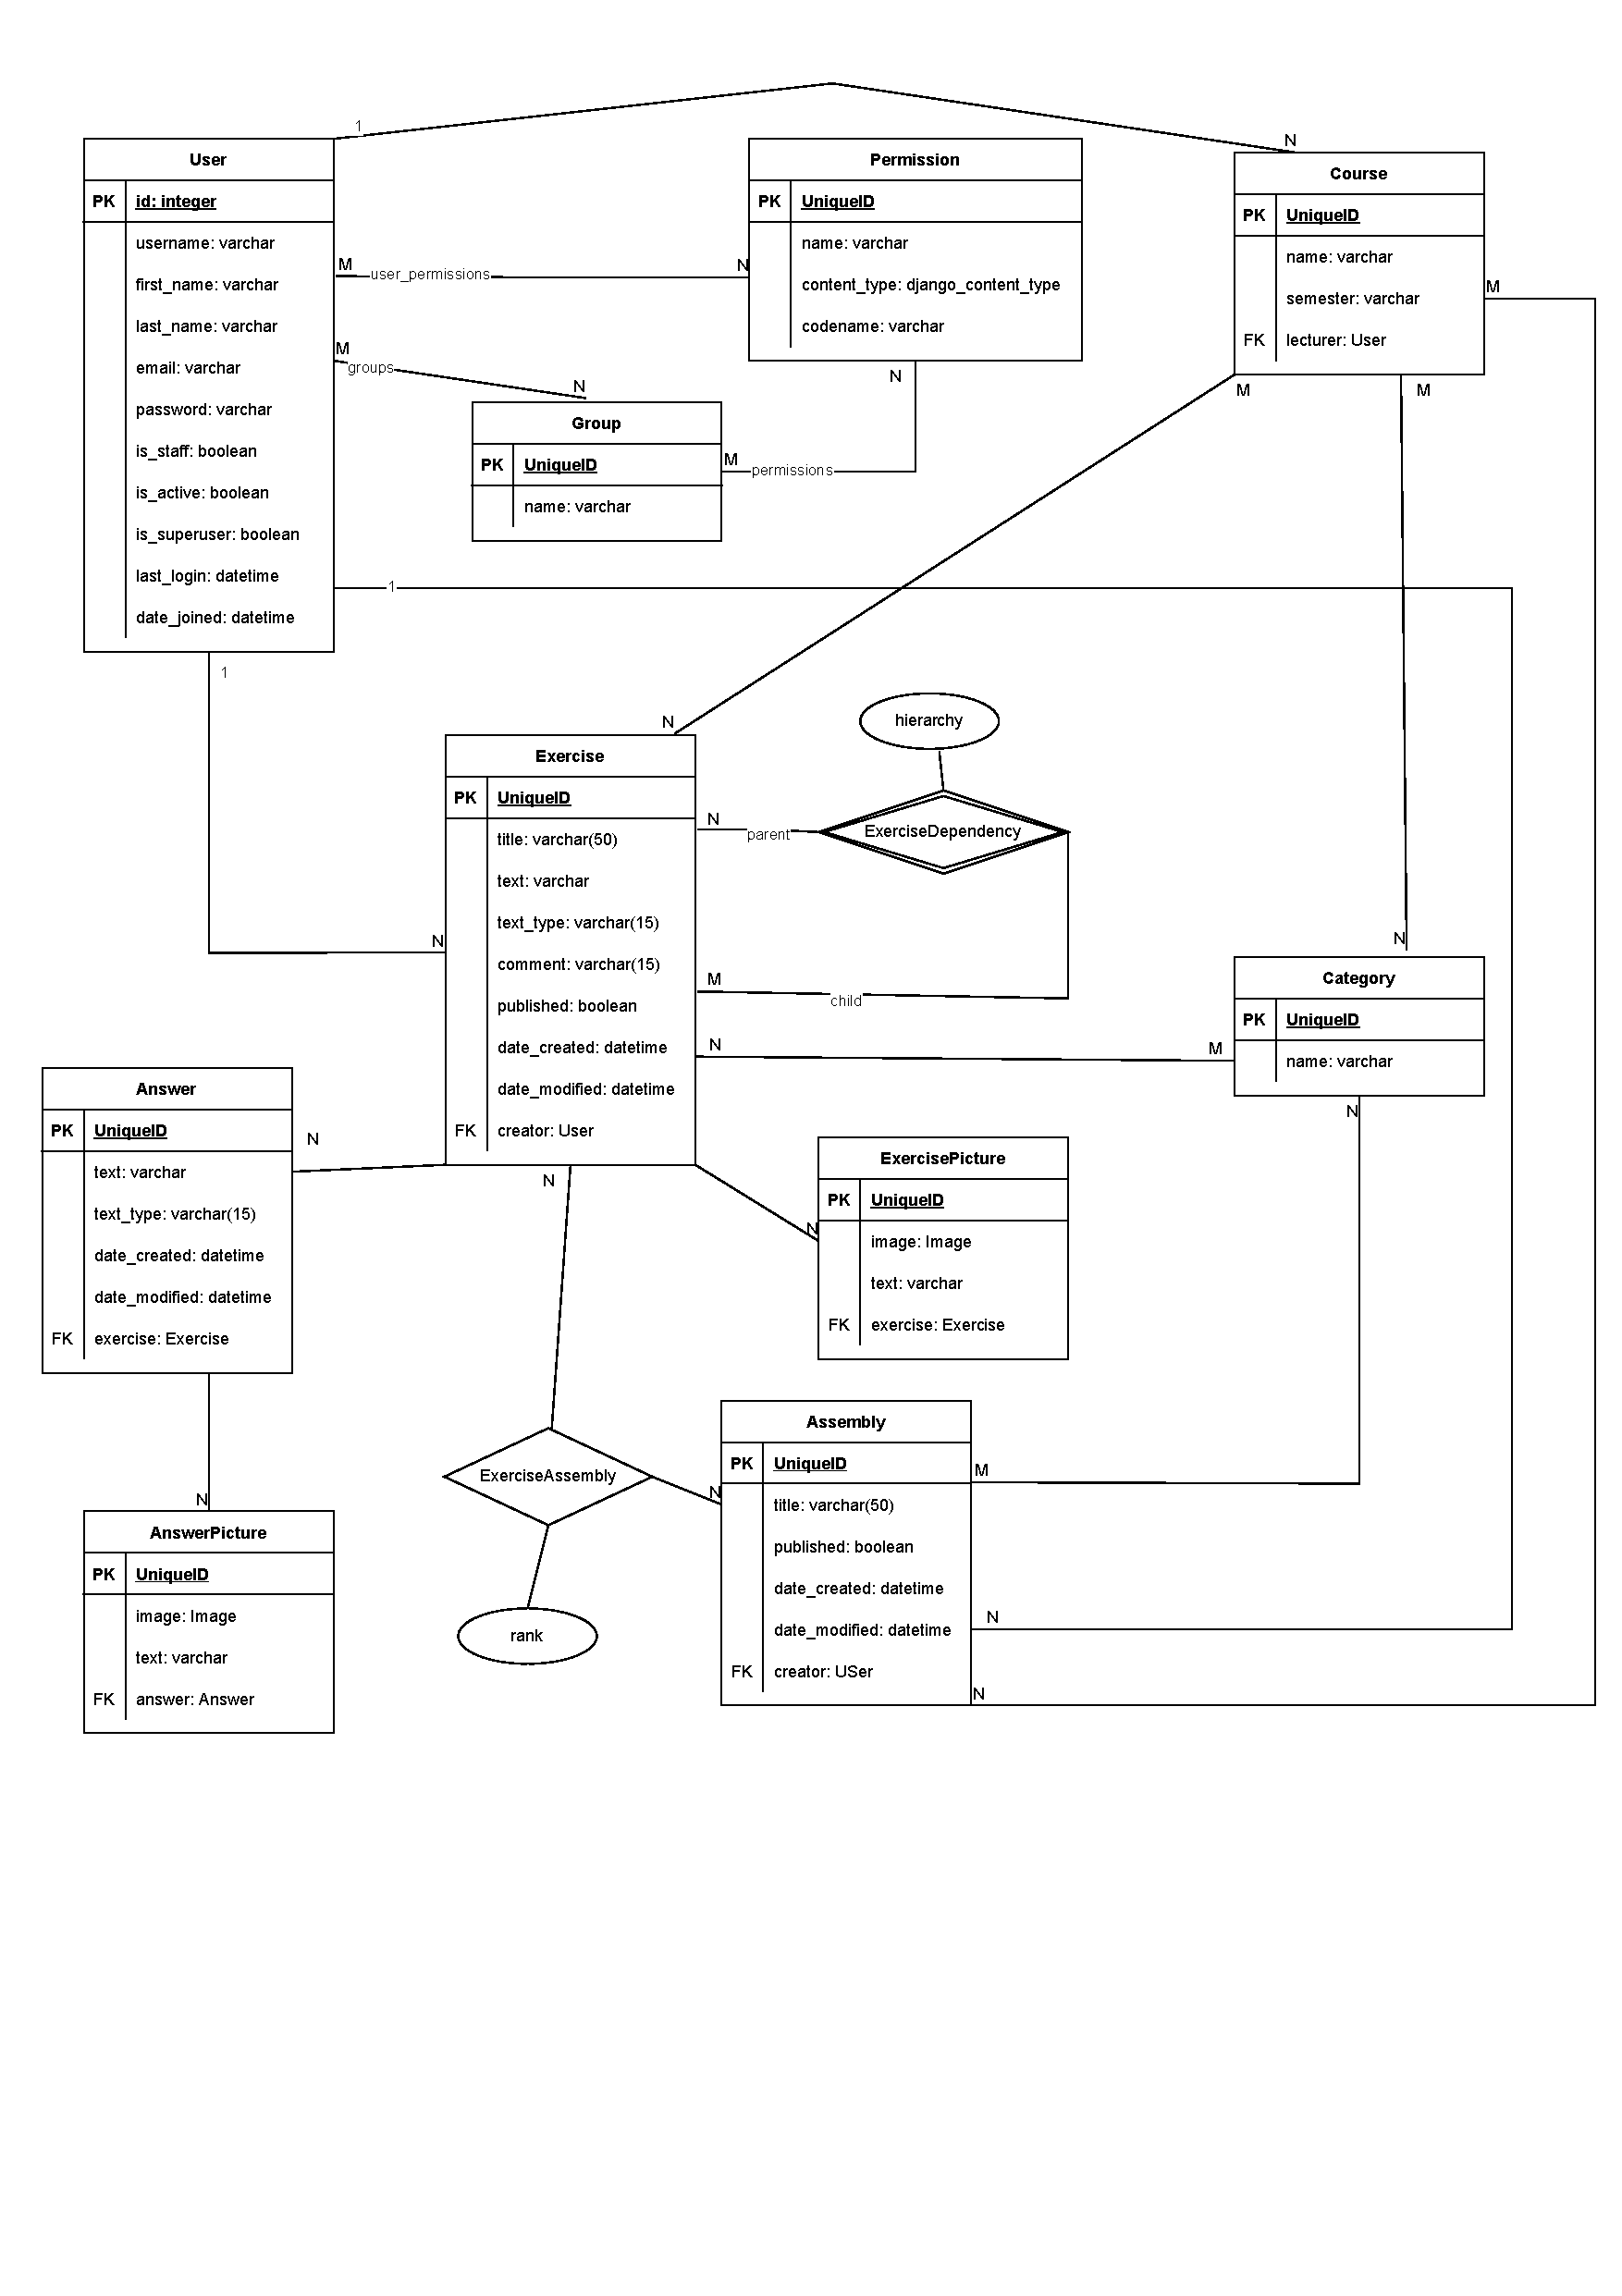
\includegraphics[height=7.5cm]{dynexgen-erd.pdf}
\end{center}
\vspace{-6mm}
\end{frame}

\begin{frame}{Pandoc}
    \begin{itemize}
        \item Dokumentenkonverter
        \item Interne Baumrepräsentation von Dokumenten
        \item Unterstützt viele Formate
        \begin{itemize}
            \item $\leftrightarrow$ \LaTeX
            \item $\leftrightarrow$ Markdown
            \item $\leftrightarrow$ HTML
            \item $\leftrightarrow$ Microsoft Word docx
            \item ($\rightarrow$ Microsoft Power Point)
            \item $\rightarrow$ PDF
        \end{itemize}
    \end{itemize}
\end{frame}

\begin{frame}{Pandoc Nachteile}
    \begin{itemize}
        \item keine Formeln in Powerpoint
        \item LaTeX Beamer macht *.tex Datein statt Folien
        \item eigene Template-Sprache
        \item eigene Datenstrukturen\\
            {\tiny \texttt{Pandoc(Meta(\{\}), [Para([Str('sei'), Space(), Str('T'), Space(), Str('ein')\dots } }
        \item weniger Kontrolle über genaues Aussehen
    \end{itemize}
\end{frame}


\begin{frame}{Backend Endpoint}
    \texttt{/generator?}\dots\\
    \quad\quad\quad\texttt{doctype=(pdf|docx|html|...)}\\
    \quad\quad\quad\texttt{\&exercise=23\&exercise=42}\\
    \quad\quad\quad\texttt{\&assembly=42}\\
    \quad\quad\quad\texttt{\&include\_answers=1\&title=0}\\
    \begin{itemize}
        \item QueryDict wird an alle Funktionen weitergereicht\\
            \quad $\Rightarrow$ einfache Konfiguration / Feature-Toggles
        \item 400 BadRequest überall möglich (via Exceptions)
        \item Content-Type für PDF, docx, odt, Text\\
            \quad $\Rightarrow$ PDF \& Text im Browser / Dokumente extern
    \end{itemize}
\end{frame}

\begin{frame}{Backend}
\begin{center}
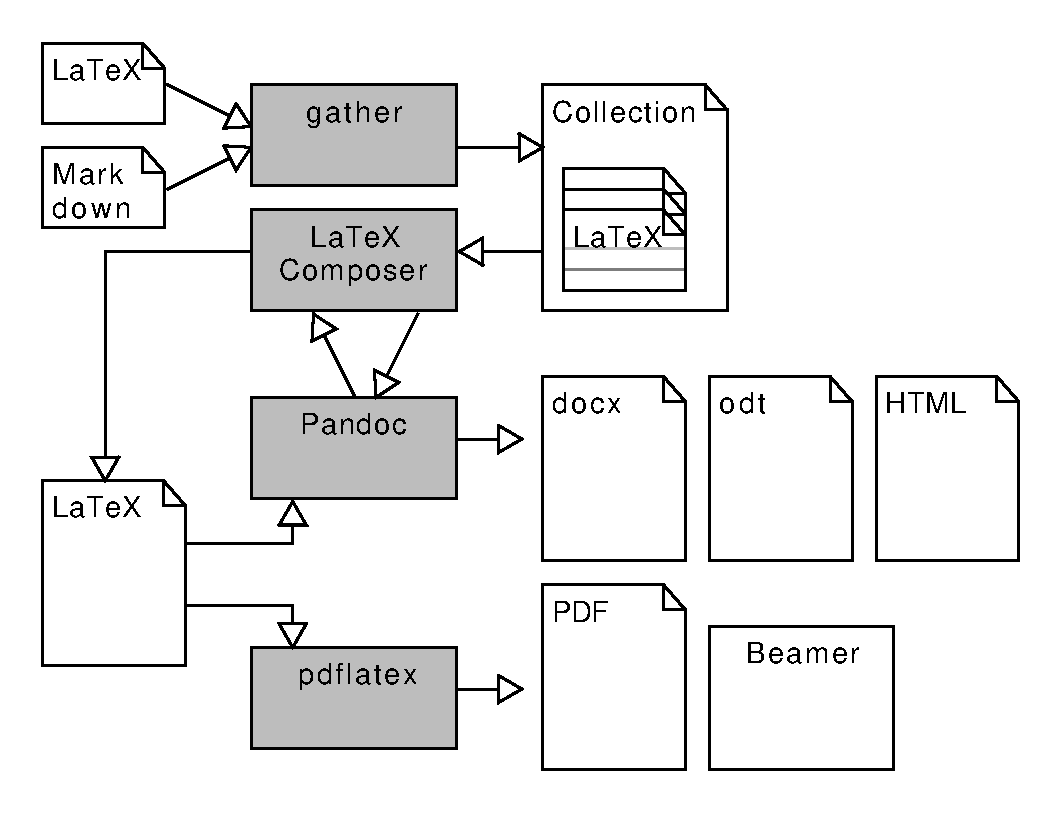
\includegraphics[height=7cm]{backend.pdf}
\end{center}
\vspace{-6mm}
\end{frame}

\end{document}
